PUT PARAMETERS
The following set of hyper-parameter values was used:
\begin{itemize}
\item C: 10\^-4:4
\item penalty: ['l2', 'l1'],
\item class\_weights': [None, 'auto']
\end{itemize}
\subsubsection{Results}
Grid search output
\begin{center}
 \begin{tabular}{ | l | c | c | c |}
   \hline
   $\bf{params_n}$ & \bf{C} &  \bf{penaly} & \bf{class\_weights} \\ \hline
   $params_1$ & 0.2682 & 'l2' & 'auto' \\ \hline
   $params_2$ & 0.2682 & 'l1' & 'auto' \\ \hline
   $params_3$ & 0.0193 & 'l2' & None \\ \hline
   $params_4$ & 0.0719 & 'l2' & 'auto' \\ \hline
   $params_5$ & 0.2682 & 'l2' & None \\ \hline
 \end{tabular}
\end{center}
\vspace{5mm}
\begin{figure}[h!]
    \centering
    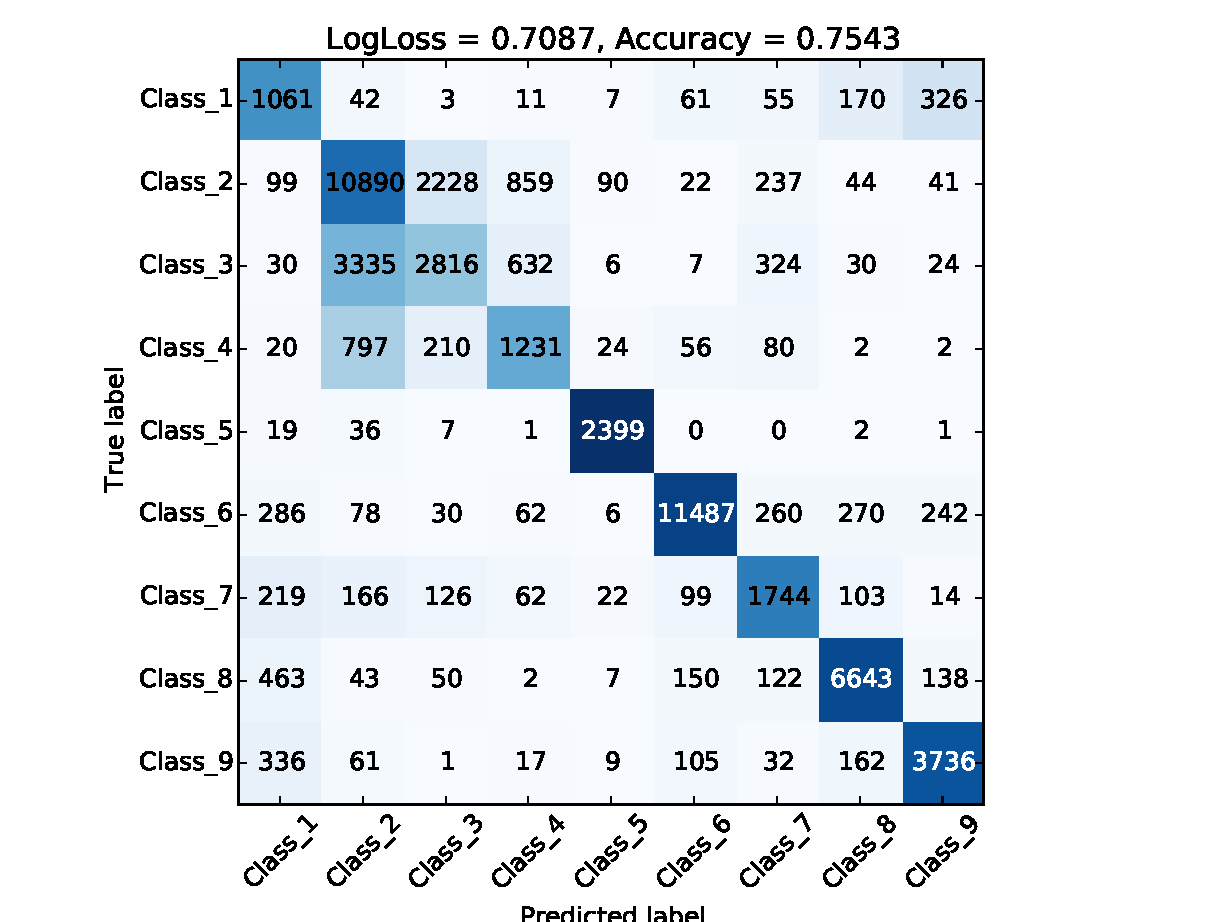
\includegraphics[width=0.8\textwidth]{LRcm_train}
    \caption{Confusion matrix using training datatset}
    \label{fig:LRcm_train}
\end{figure}\\
\begin{figure}[h!]
    \centering
    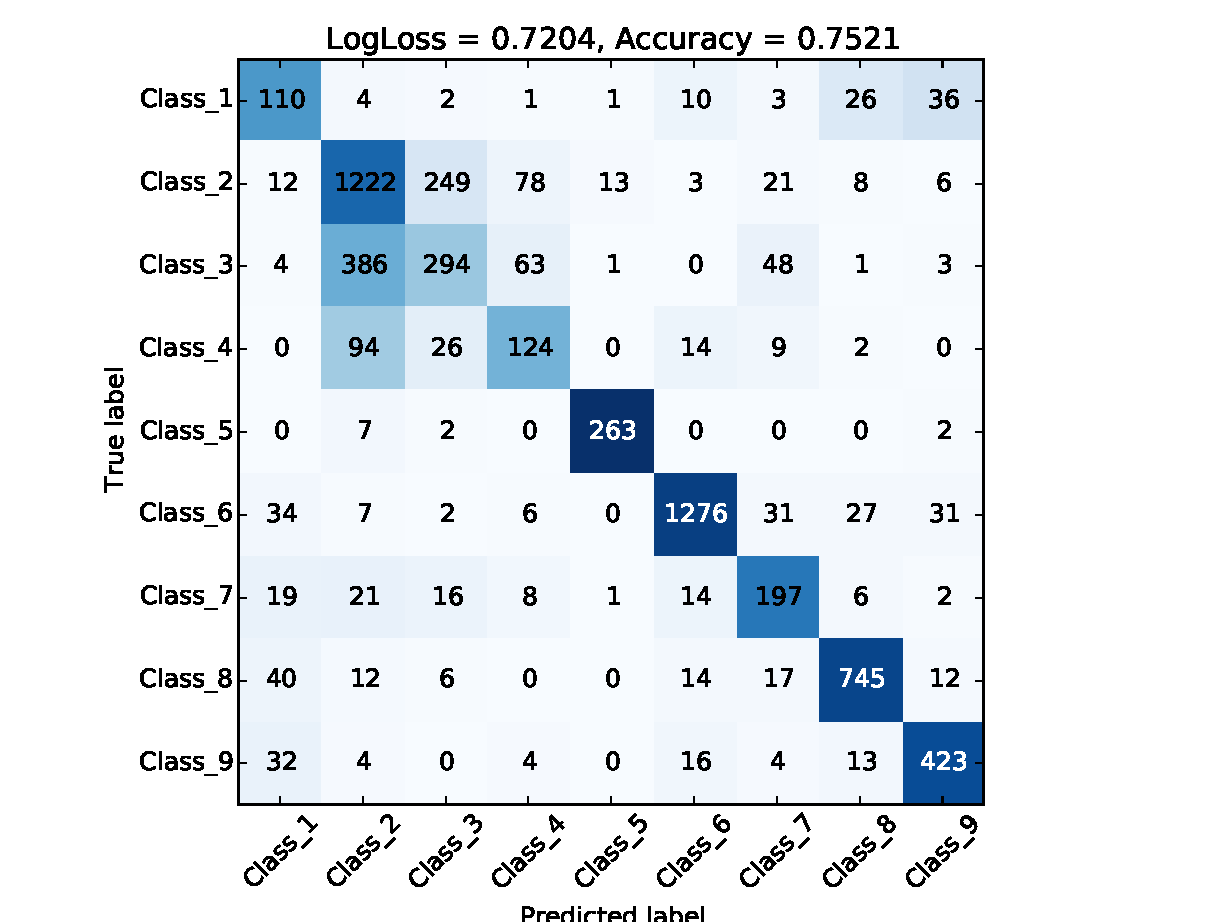
\includegraphics[width=0.8\textwidth]{LRcm_test}
    \caption{Confusion matrix using testing datatset}
    \label{fig:LRcm_test}
\end{figure}\\